\graphicspath{{chapters/04/images}}
\chapter{Materials and methods}

\section{The model}
The antennal lobe of the honey bee will be modeled as a recurrent spiking neural network.
Its architecture is based on anatomic data from the honey bee brain and modeled extending the work done on \cite{data-driven-antennal-lobe-model} and \cite{bee-geosmin}.
The implementation of the model is done in Python using the library GeNN \cite{genn}, a GPU-enhanced neural network environment based on NVIDIA CUDA \cite{cuda} technology.
GeNN offers a high-level interface to define the network architecture, the neuron and synapse models and the simulation parameters.
The Python API allows for fast development times and easy integration with other Python libraries for data analysis and visualization.
Its main advantage is the fact that the low-level CUDA code is generated automatically from a mixture of Python and C++ code, allowing it to fully exploit the power of modern GPUs without having to deal with memory management.

  \subsection{Architecture}
  A schematic representation of the architecture of the resulting spiking neural network can be seen in figure \ref{fig:al-architecture}.

  \begin{figure}
    \centering
    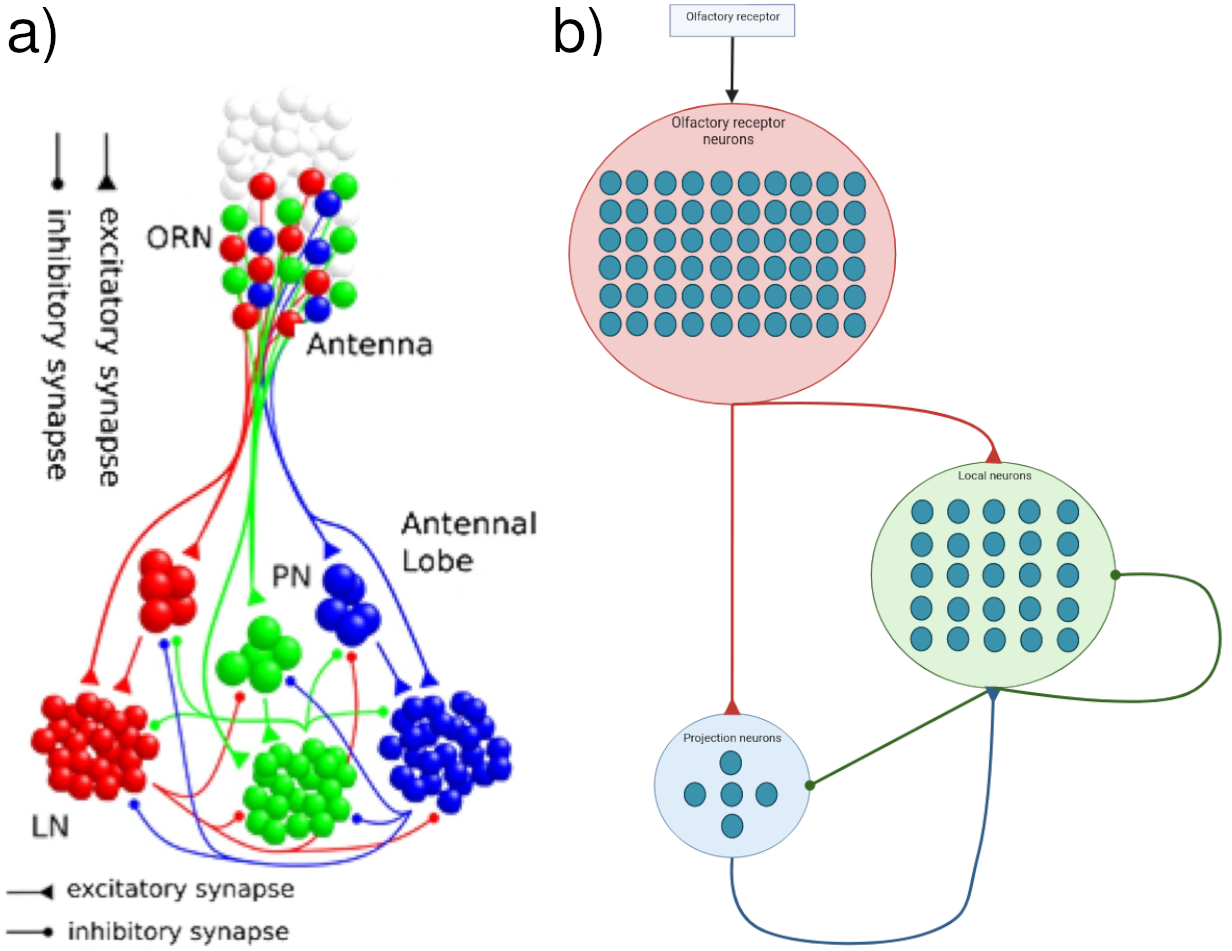
\includegraphics[width=0.8\textwidth]{al-architecture}
    \caption{\textbf{a)} Schematic representation of the architecture of the antennal lobe model. \textbf{b)} Schematic representation of the connections between neurons in a singular glomerulus.}
    \label{fig:al-architecture}
  \end{figure}

  The model is composed of $160$ glomeruli, the functional unit of the antennal lobe, which are connected to each other by the local interneurons.\\
  Each glomerulus is composed of:

  \begin{multicols}{2}
    \begin{itemize}
      \item $1$ olfactory receptor (OR).
      \item $60$ olfactory receptor neurons (ORN).
      \item $5$ projection neurons (PN).
      \item $25$ local interneurons (LN).
    \end{itemize}
  \end{multicols}

  Each glomerulus is a hierarchical structure in which the OR is connected to each neuron in the ORN population, which in turn forms excitatory synapses with PNs and LNs.
  Each neuron in the ORN population forms an excitatory synapse with a random neuron in the PN and LN populations in the same glomerulus.
  Each neuron in the PN population forms an excitatory synapse with each neuron in the LN population in the same glomerulus.
  The neurons in the LN are densely connected to each other and to neurons in the PN via inhibitory synapses.
  Communication between glomeruli is done via dense inhibitory synapses between LNs.\\
  The resulting model is a recurrent spiking neural network composed of $\numprint{14560}$ neurons and $\numprint{19220000}$ synapses.

  \subsection{Olfactory receptors}
  The olfactory receptors are the input of the model and are implemented as in \cite{bee-geosmin}.
  Biologically olfactory receptors are G-coupled protein receptors (GPCR) that bind to odorant molecules.
  They are transmembrane proteins located in the dendrites of the olfactory receptor neurons.
  When an odorant molecule binds to the receptor, it activates a G-protein which in turn activates an ionic channel, causing an increase in the membrane potential of the neuron.
  Each of the receptors is modeled to have three odor channels, so one neuron is able to be activated by three different odorants at the same time.
  Different odorants can activate the same channel, with a strength depending on their affinity to the receptor.
  The activation of the neuron is a two-step process, each of which is modeled by a differential equation.
  The first step is the binding of the odorant to the receptor:

  \begin{equation}
  \frac{dr^{(i)}_{bound}(t)}{dt} = (k_{binding}^{(i)}c_i)^nr(t) - k_{unbinding}^{(i)}r^{(i)}_{bound}(t) + k_{deactivating}^{(i)}r_{active}^{(i)}(t) - k_{activating}^{(i)}r^{(i)}_{bound}(t)
  \label{eqs:bound-receptors}
  \end{equation}

  Where:

  \begin{multicols}{2}
    \begin{itemize}
      \item $r^{(i)}_{bound}(t)$ is the fraction of channels bound by an odorant  $i$,
      \item $k_{binding}^{(i)}$ is the binding rate of odorant $i$ to the receptor.
      \item $c_i$ is the concentration of odorant $i$ receptor pair.
      \item $k_{unbinding}^{(i)}$ is the unbinding rate of the odorant $i$ receptor pair.
      \item $k_{deactivating}^{(i)}$ is the deactivation rate of the odorant $i$ receptor pair.
      \item $k_{activating}^{(i)}$ is the activation rate of the odorant $i$ receptor pair.
    \end{itemize}
  \end{multicols}

  And, in particular, the fraction of unbound receptors is computed as:

  \begin{equation}
    \frac{dr(t)}{dt} = \sum\limits_{j} k_{unbinding}^{(j)}r_{bound}^{(j)}(t) - \sum\limits_{j}(k_{binding}^{(j)}c_j)^nr(t)
  \end{equation}

  The fraction of receptors that are bound and then activated is described by:

  \begin{equation}
    \frac{dr_{active}^{(i)}(t)}{dt} = k_{activating}^{(i)} r^{(i)}_{bound}(t) - k_{deactivating}^{(i)}r_{active}^{(i)}(t)
  \end{equation}

  All the constants can be specific to the odors and receptor types.
  In this work the unbinding and deactivating rates were chosen constant and equal for all types, the binding rates were specific to the odor-receptor pair, while the activation rates were odor-specific.\\
  The total fraction of active channels can be computed as:

  \begin{equation}
    r_{active}(t) = \sum\limits_{j}r_{active}^{(j)}(t)
    \label{eqs:active-receptors}
  \end{equation}

    \subsubsection{Odors}
    \label{sec:odors}
    Odors are described by their bonding and activation rates.
    In particular, they were chosen as Gaussian profiles, as done in \cite{bee-geosmin}:

    \begin{equation}
      k_{binding}^{(i)}(j) = 10^{\eta^j}e^{-\frac{\pi^2(j)}{2*\sigma^j)^2}},\qquad j = 1, \dots, N_{glo}
    \end{equation}

    Where:

    \begin{multicols}{2}
      \begin{itemize}
        \item $\pi(\cdot)$ is a randomly chosen permutation of $1, \dots, N_{glo}$.
        \item $N_{glo}$ is the number of glomeruli in the model.
        \item $\eta\sim \mathcal{N}(1.5, 0.5^2)$ is a normally distributed random variable truncated within $\SI{0}{\kilo\hertz}$ and $\SI{4}{\kilo\hertz}$.
        \item $\sigma\sim\mathcal{N}(3, 0.5^2)$ is the standard deviation of the odor profile truncated to values greater than $\SI{1.5}{\kilo\hertz}$.
      \end{itemize}
    \end{multicols}

    The activation constant $k_{activating}^{(i)}$ was sampled from a normal distribution $\mathcal{N}(0.02, 0.02^2)$ truncated within $[\SI{0.0028}{\kilo\hertz}, \SI{0.2}{\kilo\hertz}]$.\\
    From a biological perspective, $\eta$ describes how sensitive a receptor is to an odorant, while $\sigma$ describes how broadly an odorant activates the system.

    \subsubsection{Noise}
    Bees tend to decrease their body temperature as they sleep, and this could explain the difference in the antennal lobe's activity in this state.
    To include the effects of temperature white noise has been added to the olfactory receptors, with an equation described in \cite{temperature}:

    \begin{equation}
      \sigma_j^{(i)} = \sqrt{D_j^{(i)}\cdot T \cdot \alpha}\qquad \alpha\sim\mathcal{N}(0,1)
    \end{equation}

    Where $T$ is the temperature of the system and $D_j^{(i)}$ is the $Q10$ coefficient, chosen ad hoc so the activity of the system resembles experimental data.
    $D_j^{(i)}$ is computed as:

    \begin{equation}
      D_j^{(i)} = \frac{k(T + 10)}{k(T)}\qquad k(T) = A \cdot e^{-\frac{E_a}{R\cdot T}}
    \end{equation}

    Where:

    \begin{multicols}{2}
      \begin{itemize}
        \item $A$ is a scaling factor.
        \item $R$ is the gas constant.
        \item $E_a$ is the activation energy, defined by Arrhenius equation as the minimum energy required to activate a receptor.
      \end{itemize}
    \end{multicols}

    So the new equations for the activation and binding of the odorant become:

    \begin{equation}
      \frac{dr^{(i)}_{bound}(t)}{dt} = (k_{binding}^{(i)}c_i)^nr(t) - k_{unbinding}^{(-1)}r^{(i)}_{bound} + k_{deactivating}^{(i)}r_{active}^{(i)}(t) - k_{activating}^{(i)}r^{(i)}_{bound}
    \end{equation}

    \begin{equation}
      \frac{dr_{active}^{(i)}}{dt} = k_{activating}^{(i)} r^{(i)}_{bound} - k_{deactivating}^{(i)}r_{active}^{(i)} + \sigma_{activating}^{(i)} + \sigma_{activating}^{(i)}
    \end{equation}

    \subsubsection{Effect of other brain regions}
    \label{sec:poisson-train}
    The fact that an increase in correlated activity can be seen across the whole brain during sleep \cite{slow-wave-synchronization}, suggested the possibility to add an additional correlated input into this region during sleep.
    This was done by generating for each olfactory receptor a Poisson train that will be added to the activity generated by the odor receptor following the work done in \cite{generating-poisson-train}.
    A different Poisson train was generated for each of the glomeruli via the modified next reaction method \cite{modified-next-reaction-method} algorithm (see algorithm \ref{algo:mnrm}).

    \begin{algorithm}
\DontPrintSemicolon
\SetKwComment{comment}{$\%$}{}
\SetKw{Int}{int}
\SetKw{To}{to}
\SetKw{Return}{return}
\SetKw{Not}{not}
\SetKw{Input}{Input}
\SetKw{Output}{Output}
\SetKwData{Item}{item}
\SetKwFunction{Min}{min}
\SetKwFunction{TitleFunction}{Modified Next Reaction Method (MNRM)}

\caption{\protect\TitleFunction{}}
\label{algo:mnrm}

\Input: A spike probability event accompanied by the state change variable $V_\mu$, the propensity $a$, then the initial state $V_0$ and the simulation ending time $T_{\max}$.\;

\Output: a trajectory of the membrane potetials, which is a collection of states $X(t)$ for time $0\le t\le T_{\max}$\;

$t = 0$\;
$V = V_0$\;

$T = 0$\;
generate a random number $r\sim norm(0,1)$\;
$P = \ln\frac{1}{r}$\;
compute $a$\;


\While{$t<T_{\max}$}{
	$\tau = \frac{1}{a}(P-T)$\;
	$V = V+V_\mu$\;
	$t = t+\tau$\;

	generate a random number $r\sim norm(0,1)$\;
	$P = P + \ln\frac{1}{r}$\;
	compute new $a$\;
}

\end{algorithm}


    The parameters of this algorithm were chosen to obtain biologically plausible results.\\
    After having built the Poisson trains for each of the glomeruli, a template Poisson process was generated with the same method to increase the correlation between the different glomeruli.
    Each event in the resulting trajectory of the template process was added with a probability $P_{add}$ to the Poisson train of each glomeruli and an event was removed from those latter with a probability $P_{remove}$.\\
    Each of the resulting membrane potentials was then convolved with an $\alpha$ function to obtain the final input current.
    An example of the resulting Poisson trains and the effect of adding a template can be seen in figure \ref{fig:poisson-trains}.

    \begin{figure}
      \centering
      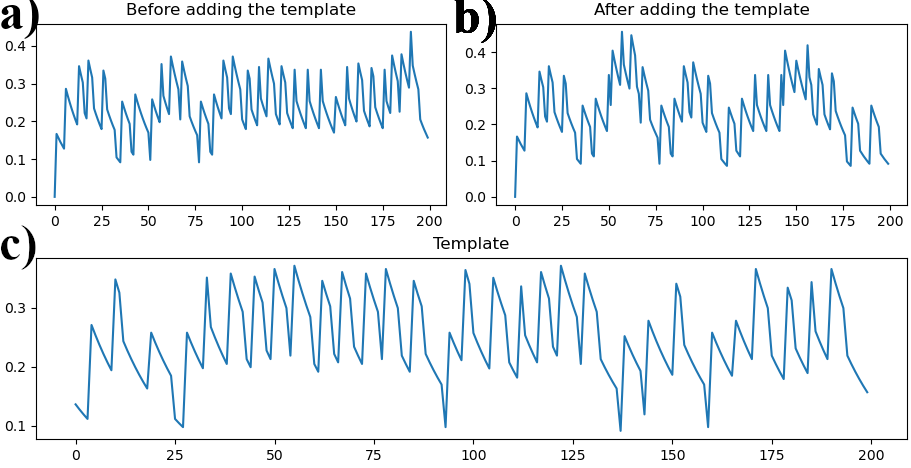
\includegraphics[width=0.8\textwidth]{poisson_train_example}
      \caption{Example of the generation of a Poisson train. \textbf{a)} A Poisson train before adding the template. \textbf{b)} The same Poisson train as in \textit{a} after adding the template. \textbf{c)} The template that is added to the other Poisson trains.}
      \label{fig:poisson-trains}
    \end{figure}

    Calling the resulting poisson train $poi$ the final activity of an olfactory receptor is computed as:

    \begin{equation}
      \frac{dr^{(i)}_{bound}(t)}{dt} = (k_{binding}^{(i)}c_i)^nr(t) - k_{unbinding}^{(-1)}r^{(i)}_{bound} + k_{deactivating}^{(i)}r_{active}^{(i)}(t) - k_{activating}^{(i)}r^{(i)}_{bound}
    \end{equation}

    \begin{equation}
      \frac{dr_{active}^{(i)}}{dt} = k_{activating}^{(i)} r^{(i)}_{bound} - k_{deactivating}^{(i)}r_{active}^{(i)} + \sigma_{activating}^{(i)} + \sigma_{activating}^{(i)} + poi^{(i)}
    \end{equation}

  \subsection{Neurons}
  The neurons in this model are described by a noisy adaptive leaky integrate and fire model.
  This model expands the classic leaky integrate and fire model by adding an adaptive term to the membrane potential:

  \begin{equation}
    I_{adapt}(t) = g_{adapt}\alpha(t)(V(t) - V_{adapt})
  \end{equation}

  This current is called adaptive because it depends on the spike train coming into the neuron.
  In particular the variable $\alpha(t)$ increases with the frequency of spikes according to:

  \begin{equation}
    \frac{d\alpha(t)}{dt} = 0.5\sum\limits_{t_{spike}}\delta(t_{spike} - t) - \frac{\alpha}{\tau_{adapt}}
  \end{equation}

  Where:

  \begin{multicols}{2}
    \begin{itemize}
      \item $\delta$ is the Dirac delta function.
      \item $\tau_{adapt}$ is the time constant of the adaptation.
    \end{itemize}
  \end{multicols}

  Other than the adaptive part the other difference from the classic leaky integrate and fire model is the noise term.
  A Gaussian noise is added to the membrane potential with the following equation:

  \begin{equation}
    noise(t) = A\sigma(t)
  \end{equation}

  Where $\sigma(i) = \mathcal{N}(0,1)\ \forall i = 0,\dots, T$ and $A$ is a constant chosen so that the noise is biologically plausible.\\
  The final equation of the membrane potential is then:

  \begin{align}
    C\frac{dV(t)}{dt} &= -I_{leak} - I_{adapt} + k I_{external} + noise(t)\\
                      &= -g_{leak}(V(t)-V_{leak}) - g_{adapt}\alpha(t)(V(t) - V_{adapt}) + k I_{external} + A\sigma(t)
    \label{eqs:neuron-model}
  \end{align}

  Where:

  \begin{multicols}{2}
    \begin{itemize}
      \item $C$ is the capacitance of the neuron.
      \item $g_{leak}$ is the conductance of the leak current.
      \item $V_{leak}$ is the reversal potential of the leak current.
      \item $g_{adapt}$ is the conductance of the adaptive current.
      \item $V_{adapt}$ is the reversal potential of the adaptive current.
      \item $k I_{external}$ is the current arriving from other neurons scaled by a factor $k$.
    \end{itemize}
  \end{multicols}

  This equation was then solved numerically using the Euler method:

  \begin{align}
    V(t + \Delta t) &= V(t) + \Delta t\frac{dV(t)}{dt}\\
                    &= V(t) + \Delta t\frac{-g_{leak}(V(t)-V_{leak}) - g_{adapt}\alpha(t)(V(t) - V_{adapt}) + k I_{external} + A\sigma(t)}{C}
  \end{align}

  And implemented in GeNN to be used in the model.

    \subsubsection{Temperature}
    The effect of temperatuer has been included also in the neurons.
    The same $Q10$ formalism has been used to change the conductances of the leak and adaptive currents:

    \begin{align}
      g_{leak}(T) &= g_{leak\ 0}(T_{ref})Q_{10}^{\frac{T - T_{ref}}{10}}
      g_{adapt}(T) &= g_{adapt\ 0}(T_{ref})Q_{10}^{\frac{T - T_{ref}}{10}}
    \end{align}

  \subsection{Synapses}
  To facilitate model implementation, the olfactory receptor, besides being a membrane protein channel, was modeled as neurons to exploit GeNN API.
  Because of this, the model presents three types of synapses:

  \begin{enumerate}
    \item Synapses between olfactory receptors and olfactory receptor neurons.
    \item Excitatory synapses between:
      \begin{itemize}
        \item Olfactory receptor neurons and projection neurons (intra-glomerulus).
        \item Projection neurons and local neurons (intra-glomerulus).
      \end{itemize}
    \item Inhibitory synapses between:
      \begin{itemize}
        \item Local neurons and projection neurons (intra-glomerulus and inter-glomerulus).
        \item Local neurons and local neurons (intra-glomerulus and inter-glomerulus).
      \end{itemize}
  \end{enumerate}

    \subsubsection{Connection between olfactory receptors and olfactory receptor neurons}
    Each olfactory receptor is connected to all the $60$ olfactory receptor neurons in the same glomerulus.
    The connection between them is modeled as a simple current injection.
    An increase in current in the olfactory receptor causes an increase in current in the olfactory receptor neuron scaled by a factor $k$:

    \begin{equation}
      I_{post\ synaptic} = k r_{active}(t)
    \end{equation}

    Where $r_{active}(t)$ is the fraction of active olfactory receptors as defined in equation \ref{eqs:active-receptors}.

    \subsubsection{Excitatory synapses}
    Each olfactory receptor neuron is connected to a random projection neuron in the same glomerulus by an excitatory synapse.
    The same is true for the connection between projection neurons and local neurons.\\
    These synapses are modeled according to a static pulse model \cite{pre-synapses}.
    In this model no learning rule is applied to the synapse and for each synapse the synaptic conductances are added to the postsynaptic input variable:

    \begin{equation}
      g_{post\ synaptic} = g_{post\ synaptic} + g_{synapse}
      \label{eqs:static-pulse}
    \end{equation}

    Where:

    \begin{multicols}{2}
      \begin{itemize}
        \item $g_{post\ synaptic}$ is the postsynaptic conductance, or $k$ in \ref{eqs:neuron-model}.
        \item $g_{synapse}$ is the conductance of the synapse, the only variable of the model.
      \end{itemize}
    \end{multicols}

    The model is then modified with an exponential decay on the conductance $g_{synapse}$.
    $g_{synapse}$ then evolves according to:

    \begin{equation}
      \frac{dg_{synapse}(t)}{dt} = -\frac{g_{synapse}(t)}{\tau_{synapse}}(V(t) - E)
      \label{eqs:exponential-decay}
    \end{equation}

    Where:

    \begin{multicols}{2}
      \begin{itemize}
        \item $\tau_{synapse}$ is the time constant of the synapse.
        \item $E$ is the reversal potential.
      \end{itemize}
    \end{multicols}


    \subsubsection{Inhibitory synapses}
    Each projection and local neuron is then connected to each local neuron both in the same and in other glomeruli.
    These synapses are modeled with the same static pulse model with exponential decay as the excitatory synapses but with different parameters for the time constant $\tau_{synapse}$ and the reversal potential $E$.\\
    Another major difference is the fact that the inhibitory synapses form dense connections: all the neurons in the source population are connected to all the neurons in the target population, instead of being connected to only one.
    Furthermore, these are the only synapses that cross the glomerulus, allowing them to communicate and synchronize the activity of the different glomeruli while introducing recurrence in the network.


\section{Data analysis}
All the data analysis was performed using Python and the following libraries:

\begin{multicols}{2}
  \begin{itemize}
    \item Pandas \cite{pandas}
    \item Numpy \cite{numpy}.
    \item Matplotlib \cite{matplotlib}.
    \item Seaborn \cite{seaborn}.
  \end{itemize}
\end{multicols}

The simulation will be performed with different parameters to fine-tune the model and make it behaves like the experimental results.
The final objective is to understand the property of the model and the behavior of the neurons in the network and understand the molecular mechanisms that cause the difference in the antennal lobe between the asleep and awake states.

  \subsection{Extracting data from a simulation}
  GeNN allows to record data from all the variables during a simulation.
  For the olfactory receptor, the data recorded is the fraction of active receptors $r_{active}(t)$.
  Then for each population of neurons, the variable recorded will be:

  \begin{multicols}{2}
    \begin{itemize}
      \item The membrane potential $V(t)$.
      \item The spike train $S(t)$.
    \end{itemize}
  \end{multicols}

  These data will then be stored in a compressed format to save space and then analyzed in an offline phase.
  The compression is performed using the Zstandard algorithm \cite{zstandard}.\\
  This has been chosen because it is a fast lossless compression algorithm, built specifically for real-time compression scenarios while achieving better compression ratios.
  This is important because the simulation will be performed on a cluster of GPU nodes and the data will be stored on a shared file system.
  Optimizing the space used by the data will allow to store more data and perform more simulations.

  \subsection{Neuron's activity}
  The evolution of the membrane potential $V(t)$ of a neuron is a good indicator of the activity of the neuron.
  Because of this it will be recorded and then, to allow for a visualization of the activity of the network, it will be plotted using Matplotlib \cite{matplotlib}.
  Because there are too many neurons to allow for a visualization of the activity of each neuron, only a random neuron in the most active glomerulus will be plotted for each population.\\
  This type of plot will give information about the general activity of the neurons in each population and will allow to see if the network is behaving as expected.

  \subsection{Spike density matrix}
  The spike density matrix will show the average firing rates of all the glomeruli in the network.
  The spike train for each neuron of each population in a network is collected from the simulation and then it is convolved with a Gaussian kernel to obtain the firing rate of each neuron.
  The firing rates of the neurons are then averaged across population and glomeruli and plotted as a heatmap using Matplotlib \cite{matplotlib}.\\
  This type of plot will give information about the activity of the population of neurons per glomeruli, giving visual information about which glomerulus is activated by a specific odor, or how the input is transformed when it travels across the populations of neurons.

  \subsection{Correlation matrices}
  The correlation matrices are built using the spike density matrix as obtained in the previous sections.
  In this way, the correlation of the firing rates of neurons in the same population per glomerulus can be visualized.\\
  It is computed using the \texttt{corrcoef} function of Numpy \cite{numpy} (equation \ref{eqs:corrcoef}).

  \begin{equation}
    R_{ij} = \frac{C_{ij}}{\sqrt{C_{ii}C_{jj}}}
    \label{eqs:corrcoef}
  \end{equation}

  Where $C_{ij}$ is the covariance matrix of the input matrix:

  \begin{equation}
    C_{ij} = \frac{1}{n-1}\sum_{k=1}^{n}(X_{ki} - \bar{X_i})(X_{kj} - \bar{X_j})
  \end{equation}

  This function takes as input the spike density matrix and returns the Pearson product-moment correlation coefficient.
  In particular it returns a matrix $C$ where $C_{i,j}$ is the correlation coefficient between the $i$-th and the $j$-th column of the input matrix such that:

  \begin{itemize}
    \item $C_{i,j} > 1$ the activity of the two glomeruli is positively correlated.
    \item $C_{i,j} = 0$ the activity of the two glomeruli is not correlated.
    \item $C_{i,j} < 0$ the activity of the two glomeruli is negatively correlated.
  \end{itemize}

  The resulting correlation matrix is then clustered using the \texttt{linkage} function of Scipy \cite{scipy} with the \texttt{complete} method and plotted as heatmap using Seaborn \cite{seaborn}.
  Clustering is performed with a hierarchichal and agglomerative algorithm and the distance used is the Farthest Point Algorithm or Voorhees Algorithm \cite{fpa}.
  This type of plot is of fundamental importance because one of the most visible effects of sleep in experimental data is an increase in the correlation between the projection neurons across glomeruli with respect to the awake state.

  \subsection{Feature extraction}
  \label{sec:feature-extraction}
  After having fine-tuned the model so it reproduces the experimental data obtained from observing the activity of the antennal lobe of a bee in the awake and asleep state, the model will be used to extract features from the data.\\
  This is done because from the experimental data it was noticed that there were no significant changes in the average firing rate of the observed brain regions, but what changed was, besides the increase in correlation, network-level features.\\
  Several features will be extracted and analyzed using the Python library bct \cite{bct}.
  Bct is a brain connectivity toolbox for Matlab, but it has been ported to Python and it is available as a pip package.
  It provides several graph theoretical measures, and it will be used to extract several connectivity features.
  Besides the connectivity features, other features will be extracted from the data, regarding the distribution of the activity of the neurons in the network.\\
  The various features will be compared visually thanks to Seaborn's \cite{seaborn} \texttt{pairplot} function.

    \subsubsection{Distribution features}
    The distribution features will be extracted using a combination of the Scipy \cite{scipy}, Numpy \cite{numpy} and Nolds \cite{nolds} libraries.

      \paragraph{Standard deviation}
      \label{sec:std}
      The standard deviation of the activity of the neurons in the network is computed as the average of the standard deviation of the activity of neurons at each timestep.
      For a single timestep the standard deviation is computed as:

      \begin{equation}
        \sigma = \sqrt{\frac{1}{N}\sum_{i=1}^{N}(x_i - \mu)^2}
      \end{equation}

      Where:

      \begin{itemize}
        \item $N$ is the number of neurons in the network.
        \item $x_i$ is the activity of the $i$-th neuron.
        \item $\mu$ is the average activity of the neurons in the network.
      \end{itemize}

      \paragraph{Skewness}
      \label{sec:skewness}
      The skewness of the activity of the neurons in the network is computed as the average of the skewness of the activity of neurons at each timestep.
      For a single timestep the skewness is computed as the Fisher-Pearson coefficient of skewness:

      \begin{equation}
        g_1 = \frac{m_3}{m_2^{3/2}}\qquad m_i = \frac{1}{N}\sum_{i=1}^{N}(x_i - \mu)^i
      \end{equation}

      Where:

      \begin{itemize}
        \item $N$ is the number of neurons in the network.
        \item $x_i$ is the activity of the $i$-th neuron.
        \item $\mu$ is the average activity of the neurons in the network.
      \end{itemize}

      \paragraph{Kurtosis}
      \label{sec:kurtosis}
      The kurtosis of the activity of the neurons in the network is computed as the average of the kurstosis of the activity of neurons at each timestep.
      For a single timestep the kurtosis is the fourth central momen divided by the square of the variance:

      \begin{equation}
        \beta_2 = \frac{\mu^4}{\sigma^4}
      \end{equation}

      \paragraph{Sample entropy}
      \label{sec:sampen}
      The sample entropy of the activity of the neurons in the network is computed as the average of the kurstosis of the activity of neurons at each timestep.
      For a single timestep the sample entropy is the negative natural logarithm of the conditional probability that two sequences remain similar at the next point in the activity's time series.
      It is computed by constructing all subsequences of length $m$ and count all different pairs distant less than a predefined threshold $r$.
      The same is done for all subsequences of length $m+1$.
      Then the sum of similar sequence pairs with length $m+1$ is divided by the sum of similar sequence pairs with length $m$.
      The result is then the negative logarithm of this probability.

      \paragraph{Hurst exponent}
      \label{sec:hurst}
      The Hurst exponent of the activity of the neurons in the network is computed as the average of the kurstosis of the activity of neurons at each timestep.
      It is a measure of long-term memory of the activity time series: the long statistical dependencies in the data that do not originate from cycles.
      It is computed by subtracting the mean from the time series and computing the cumulative sum of the resulting time series.
      Then the cumulative sum is divided into $N$ non-overlapping segments of equal length.

      \paragraph{Detrended fluctuation analysis}
      \label{sec:dfa}
      The detrended fluctuation analysis (DFA) is a method that will be used to find long-term statistical dependencies in the time series of the activity of neurons, similarly to the Hurst exponent.
      It is computed for a single timestep by dividing the time series into $N$ non-overlapping segments of equal length.
      Then for each segment the trend is removed by subtracting the least squares fit of the data in the segment.
      Then the root mean square of the data in each segment is computed.
      Finally the root mean square is plotted against the length of the segment in a log-log plot and the slope of the resulting line is the DFA.

    \subsubsection{Connectivity features}
    Connectivity features focus on the network-level effect rather than on the time series of the data.
    These features will be extracted from the functional connectivity of the network, which depends on the activity of the neurons in the network, rather than its architecture.
    Functional connectivity is extracted by computing the Pearson coefficient of the time series of the activity for each pair of neurons in the network.
    If the coefficient is greater than a threshold a functional connection is found between the neurons, otherwise there is no functional connection.\\
    The features will be extracted using the library bct \cite{bct} and will be:


      \paragraph{Betweenness centrality}
      \label{sec:betweenness}
      The betweenness centrality of a node is the average fraction of all shortest paths in the network that contain a given node.
      It is computed through Kintali's algorithm \cite{betweenness}.

      \paragraph{Transitivity}
      \label{sec:transitivity}
      The transitivity  is the ratio of triangles to triplets in the network.
      From a connectivity graph it counts the triangles and the triplets and then divides the triangles by the triplets.

      \paragraph{Degree}
      \label{sec:degree}
      The degree is the average number of incoming and outgoing links connected to a node.

      \paragraph{Efficiency}
      \label{sec:efficiency}
      The efficiency is the average of inverse shortest path length.
      It is inversely related to the characteristic path length.

      \paragraph{Frobenius norm}
      \label{sec:norm}
      The Frobenius norm is the square root of the sum of the aboslute squares of its elements.
      It is a measure of the size of a matrix.
      It is computed for the adjacency matrix of the connectivity graph as:

      \begin{equation}
        ||A||_F = \left[\sum\limits_{i,j}|a_{ij}|^2\right]^{1/2}
      \end{equation}
